\documentclass[IJ]{cesj}
\usepackage{graphicx}
\usepackage{listings}

\author{Ga\"etan Lehmann}
\institute{Biologie du d\'eveloppement et de la reproduction, INRA de Jouy-en-Josas}

\title{MorphologicalGradientImageFilter}
\abstract{Morphological gradients enhance the variation of pixel intensity in a given neighborhood.}
\keyword{mathematical morphology, gradient}
\year{2005}

\leftmark{Ga\"etan Lehmann}
\rightmark{Ga\"etan Lehmann}

\begin{document}
\lstset{language=c++}
\maketitle
% \tableofcontents

\section{Description}
Morphological gradients enhance the variation of pixel intensity in a given neighborhood. This filter can be used to produce the basic morphological gradient (aka Beucher's gradient), the thick gradient and the directionnal gradient, depending of the size and the shape of structuring element.

\section{Implementation}
MorphologicalGradientImageFilter is a mini pipeline with a GrayscaleDilateImageFilter, a GrayscaleErodeImageFilter and a SubtractImageFilter. A lots more efficient implementation should be done by doing the erosion the dilation and the subtraction in the same pass. It should be easy and efficent to that with a moving histogram algorithm (not ready yet).

\section{Usage}
As usual, user has to include the header:
\begin{lstlisting}
#include "itkMorphologicalGradientImageFilter.h"
#include "itkBinaryBallStructuringElement.h"
\end{lstlisting}
Create the structuring element\footnote{Creating a structuring element is mandatory, even if a good default behavior would have be to use a structuring element of radius one. This problem is related to bug \#1877.}.
\begin{lstlisting}
typedef itk::BinaryBallStructuringElement< PType, dim >
  StructuringElementType;
StructuringElementType  structuringElement;
structuringElement.SetRadius( 2 );
structuringElement.CreateStructuringElement();
\end{lstlisting}
Create the filter
\begin{lstlisting}
typedef itk::MorphologicalGradientImageFilter
  < IType, IType, StructuringElementType > GradientType;
GradientType::Pointer gradient = GradientType::New();
gradient->SetInput( filter->GetOutput() );
gradient->SetKernel( structuringElement );
\end{lstlisting}


\section{Example}
\begin{figure}[b]
\centering

\includegraphics[width=0.5\textwidth]{cthead1.eps}
\caption{The input image.}
\end{figure}

\begin{figure}
\centering
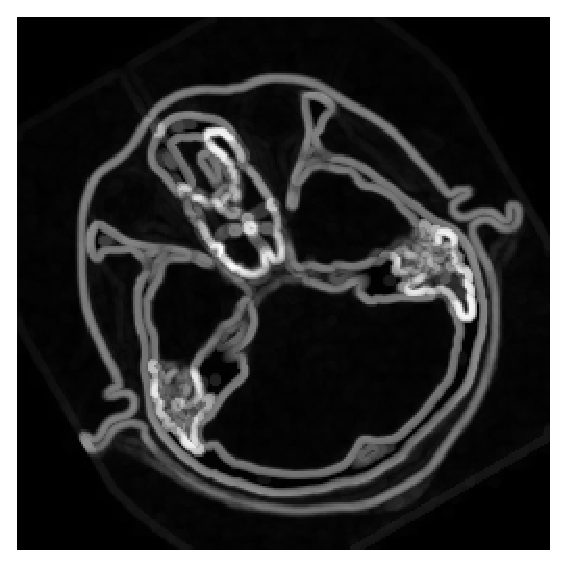
\includegraphics[width=0.5\textwidth]{gradient.eps}
\caption{The gradient image.}
\end{figure}

\end{document}
